\documentclass{article}
\usepackage{tikz}
\usetikzlibrary{shapes.geometric, arrows}

\tikzstyle{startstop} = [rectangle, rounded corners, 
minimum width=3cm, 
minimum height=1cm,
text centered, 
draw=black, 
fill=red!30]

\tikzstyle{io} = [trapezium, 
trapezium stretches=true, % A later addition
trapezium left angle=70, 
trapezium right angle=110, 
minimum width=3cm, 
minimum height=1cm, text centered, 
draw=black, fill=blue!30]

\tikzstyle{process} = [rectangle, 
minimum width=3cm, 
minimum height=1cm, 
text centered, 
text width=3cm, 
draw=black, 
fill=orange!30]

\tikzstyle{decision} = [circle, 
minimum width=0.1cm, 
minimum height=0.1cm, 
text centered, 
draw=black, 
fill=green!30]
\tikzstyle{arrow} = [thick,->,>=stealth]
\begin{document}
\noindent\hspace*{-2cm}%
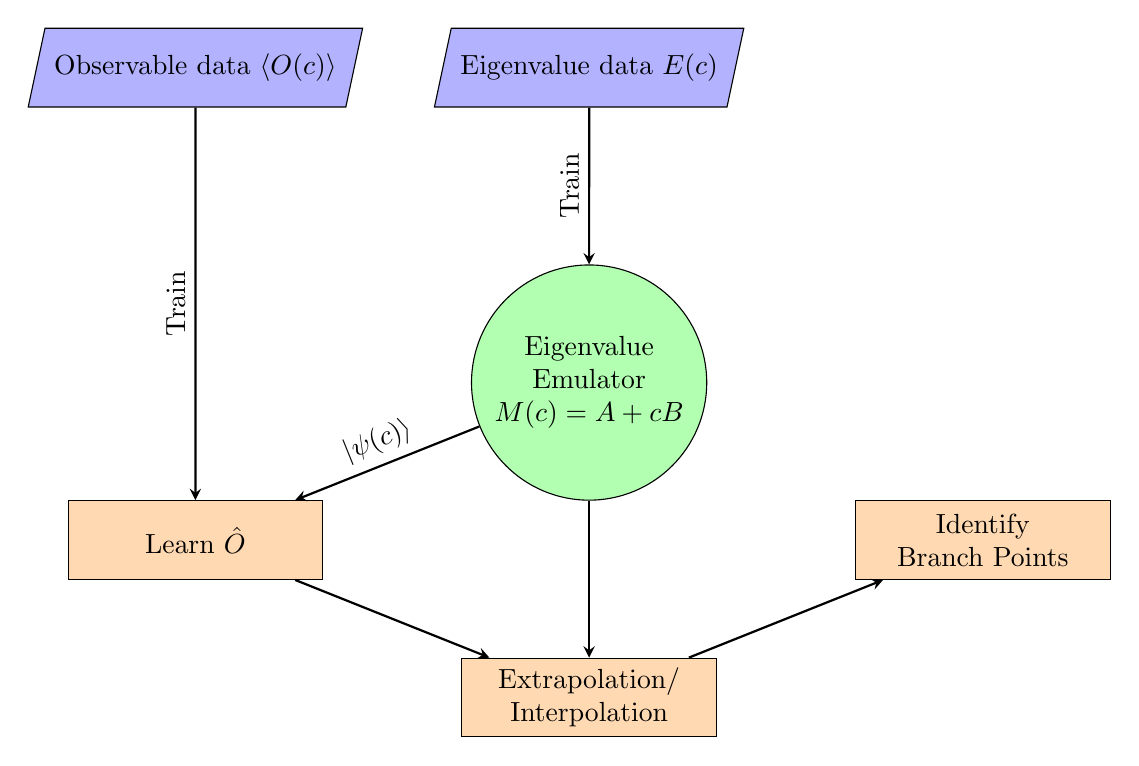
\begin{tikzpicture}[node distance=2cm]

% \node (start) [startstop] {Hamiltonian $H(c)$};
\node (in1) [io] {Eigenvalue data $E(c)$};
\node (in2) [io, left of=in1, node distance=5cm] {Observable data $\langle O(c)\rangle$};
\node (MEE) [decision, below of=in1,yshift=-2cm, align=center]{Eigenvalue\\ 
Emulator \\
$M(c) = A+cB$};
\node (ET) [process, below of=MEE, yshift=-2cm] {Extrapolation/
Interpolation};
\node (obv) [process, below of=MEE, xshift=-5cm] {Learn $\hat{O}$};
\node (branch) [process, right of=obv, xshift=8cm] {Identify Branch Points};

% \draw [arrow] (start) -- (in1);
% \draw [arrow] (start) --node[anchor=west,xshift=0.5cm]{}(in2);
\draw [arrow] (in1) -- node[anchor=south,rotate=90] {Train} (MEE);
\draw [arrow] (in2) -- node[anchor=south,rotate=90]{Train} (obv);
\draw [arrow] (MEE) -- node[anchor=south,rotate=22] {$|\psi(c)\rangle$}(obv);
\draw [arrow] (MEE) -- (ET);
% \draw [arrow] (MEE) -- (branch);
\draw [arrow] (obv) -- (ET);
\draw [arrow] (ET) -- (branch);

\end{tikzpicture}
\end{document}